\documentclass{amsart}
\usepackage{amssymb}
\renewcommand{\baselinestretch}{1.5}
\addtolength{\textwidth}{.2in}
\addtolength{\topmargin}{-.5in}
\addtolength{\textheight}{1in}

\usepackage{ifthen}
\usepackage{graphicx}

\newcommand{\versionNum}{$3.2$\ }

\newboolean{InTextBook}
\setboolean{InTextBook}{false}
\newboolean{InWorkBook}
\setboolean{InWorkBook}{false}
\newboolean{InHints}
\setboolean{InHints}{false}

%When this boolean is true (beginning in Section 5.1) we will use the convention
% that $0 \in \Naturals$.  If it is false we will continue to count $1$ as the smallest
%natural number (thus making Giuseppe Peano spin in his grave...)
 
\newboolean{ZeroInNaturals}

%This boolean is used to distinguish the version where we use $\sim$ rather than $\lnot$

\newboolean{LNotIsSim}

%The values of the last two booleans are set in ``switches.tex''

\setboolean{ZeroInNaturals}{true}
\setboolean{LNotIsSim}{false}


\let\savedlnot\lnot
\ifthenelse{\boolean{LNotIsSim}}{\renewcommand{\lnot}{\sim} }{}

%This command puts different amounts of space depending on whether we are
% in the text, the workbook or the hints & solutions manual. 
\newcommand{\twsvspace}[3]{%
 \ifthenelse{\boolean{InTextBook} }{\vspace{#1}}{%
  \ifthenelse{\boolean{InWorkBook} }{\vspace{#2}}{%
   \ifthenelse{\boolean{InHints} }{\vspace{#3}}{} %
   }%
  }%
 }


\newcommand{\wbvfill}{\ifthenelse{\boolean{InWorkBook}}{\vfill}{}}
\newcommand{\wbitemsep}{\ifthenelse{\boolean{InWorkBook} }{\rule[-24pt]{0pt}{60pt}}{}}
\newcommand{\textbookpagebreak}{\ifthenelse{\boolean{InTextBook}}{\newpage}{}}
\newcommand{\workbookpagebreak}{\ifthenelse{\boolean{InWorkBook}}{\newpage}{}}
\newcommand{\hintspagebreak}{\ifthenelse{\boolean{InHints}}{\newpage}{}}

\newcommand{\hint}[1]{\ifthenelse{\boolean{InHints}}{ {\par \hspace{12pt} \color[rgb]{0,0,1} #1 } }{}}
\newcommand{\inlinehint}[1]{\ifthenelse{\boolean{InHints}}{ { \color[rgb]{0,0,1} #1 } }{}}

\newlength{\cwidth}
\newcommand{\cents}{\settowidth{\cwidth}{c}%
\divide\cwidth by2
\advance\cwidth by-.1pt
c\kern-\cwidth
\vrule width .1pt depth.2ex height1.2ex
\kern\cwidth}

\newcommand{\sageprompt}{ {\tt sage$>$} }
\newcommand{\tab}{\rule{20pt}{0pt}}
\newcommand{\blnk}{\rule{1.5pt}{0pt}\rule{.4pt}{1.2pt}\rule{9pt}{.4pt}\rule{.4pt}{1.2pt}\rule{1.5pt}{0pt}}
\newcommand{\suchthat}{\; \rule[-3pt]{.5pt}{13pt} \;}
\newcommand{\divides}{\!\mid\!}
\newcommand{\tdiv}{\; \mbox{div} \;}
\newcommand{\restrict}[2]{#1 \,\rule[-4pt]{.25pt}{14pt}_{\,#2}}
\newcommand{\lcm}[2]{\mbox{lcm} (#1, #2)}
\renewcommand{\gcd}[2]{\mbox{gcd} (#1, #2)}
\newcommand{\Naturals}{{\mathbb N}}
\newcommand{\Integers}{{\mathbb Z}}
\newcommand{\Znoneg}{{\mathbb Z}^{\mbox{\tiny noneg}}}
\ifthenelse{\boolean{ZeroInNaturals}}{%
  \newcommand{\Zplus}{{\mathbb Z}^+} }{%
  \newcommand{\Zplus}{{\mathbb N}} }
\newcommand{\Enoneg}{{\mathbb E}^{\mbox{\tiny noneg}}}
\newcommand{\Qnoneg}{{\mathbb Q}^{\mbox{\tiny noneg}}}
\newcommand{\Rnoneg}{{\mathbb R}^{\mbox{\tiny noneg}}}
\newcommand{\Rationals}{{\mathbb Q}}
\newcommand{\Reals}{{\mathbb R}}
\newcommand{\Complexes}{{\mathbb C}}
%\newcommand{\F2}{{\mathbb F}_{2}}
\newcommand{\relQ}{\mbox{\textsf Q}}
\newcommand{\relR}{\mbox{\textsf R}}
\newcommand{\nrelR}{\mbox{\raisebox{1pt}{$\not$}\rule{1pt}{0pt}{\textsf R}}}
\newcommand{\relS}{\mbox{\textsf S}}
\newcommand{\relA}{\mbox{\textsf A}}
\newcommand{\Dom}[1]{\mbox{Dom}(#1)}
\newcommand{\Cod}[1]{\mbox{Cod}(#1)}
\newcommand{\Rng}[1]{\mbox{Rng}(#1)}

\DeclareMathOperator\caret{\raisebox{1ex}{$\scriptstyle\wedge$}}

\newtheorem*{defi}{Definition}
\newtheorem*{exer}{Exercise}
\newtheorem{thm}{Theorem}[section]
\newtheorem*{thm*}{Theorem}
\newtheorem{lem}[thm]{Lemma}
\newtheorem*{lem*}{Lemma}
\newtheorem{cor}{Corollary}
\newtheorem{conj}{Conjecture}

\renewenvironment{proof}%
{\begin{quote} \emph{Proof:} }%
{\rule{0pt}{0pt} \newline \rule{0pt}{15pt} \hfill Q.E.D. \end{quote}}


\addtolength{\abovedisplayskip}{0pt}
\addtolength{\belowdisplayskip}{24pt}
\addtolength{\abovedisplayshortskip}{0pt}
\addtolength{\belowdisplayshortskip}{48pt}


\begin{document}
\thispagestyle{empty}

\centerline{\Large Activity 22 -- Introduction to Proof}
\centerline{\large set operations}

\bigskip
\Large


\begin{enumerate}

\item Calculate the union and intersection of $\{1, 2, 3, 5 \}$ and $\{ 1, 3, 4, 5 \}$.

\vfill

\item Let $A = \{1, 2, 3, 4, 5, 6, 7 \}$ and $B = \{2, 4, 6, 8, 10\}$. Calculate the following:

\vspace{.2in}

\begin{enumerate}
\item $A \setminus B \; = $

\vspace{.2in}

\item $B \setminus A \; = $

\vspace{.2in}

\item $A \triangle B \; = $

\vspace{.2in}

\item $A \cup B \; = $

\vspace{.2in}

\item $A \cap B \; = $

\vspace{.2in}

\item $(A \cup B) \, \setminus \, (A \cap B) \; = $

\vspace{.7in}

\end{enumerate}

\item Suppose $U = \{1, 2, \ldots 10 \}$.  Let $A = \{1, 4, 6, 8, 9, 10 \}$.  What is $\overline{A}$?

\vfill

\newpage

\item (Exercise 2 in \S 4.3 of GIAM) In a standard deck of playing cards one can distinguish sets
based on face-value and/or suit.  Let $A, 2, \ldots 9, 10, J, Q$ and $K$
represent the sets of cards having the various face-values.  Also, let
$\heartsuit$, $\spadesuit$, $\clubsuit$ and $\diamondsuit$ be the 
sets of cards having the possible suits.  Find the following
  \begin{enumerate}
  \item \rule[-18pt]{0pt}{48pt}$A \cap \heartsuit$ 
  \item \rule[-18pt]{0pt}{48pt}$A \cup \heartsuit$ 
  \item \rule[-18pt]{0pt}{48pt}$J \cap (\spadesuit \cup \heartsuit)$ 
  \item \rule[-18pt]{0pt}{48pt}$K \cap \heartsuit$ 
  \item \rule[-18pt]{0pt}{48pt}$A \cap K$ 
  \item \rule[-18pt]{0pt}{48pt}$A \cup K$ 
  \end{enumerate}

\vspace{.7in}

\item Let $A = \{1, 2, 3, 4, 5, 6, 7 \}$ and $B = \{2, 4, 6, 8, 10\}$. (The same sets as in problem 2.)  Calculate all of the elements in DeMorgan's law: $\overline{A \cup B}$ and $\overline{A}$ and $\overline{B}$ and $\overline{A} \cap \overline{B}$.

\vfill

\newpage

\item (Exercise 3 in \S 4.3 of GIAM) The following is a screenshot from the computational geometry program OpenSCAD (very handy for making models for 3-d printing\ldots)  In computational geometry we use the basice set operations together
with a few other types of transformations to create interesting models using simple components.  Across the top of the image below we see 3 sets of points in $\Reals^3$, a ball, a sort of 3-dimensional plus sign, and a disk.  Let's call the ball $A$, the plus sign $B$ and the disk $C$.   The nine shapes shown below them are made from $A$, $B$ and $C$ using union, intersection and set difference.  Identify them!

\vspace{.5in}
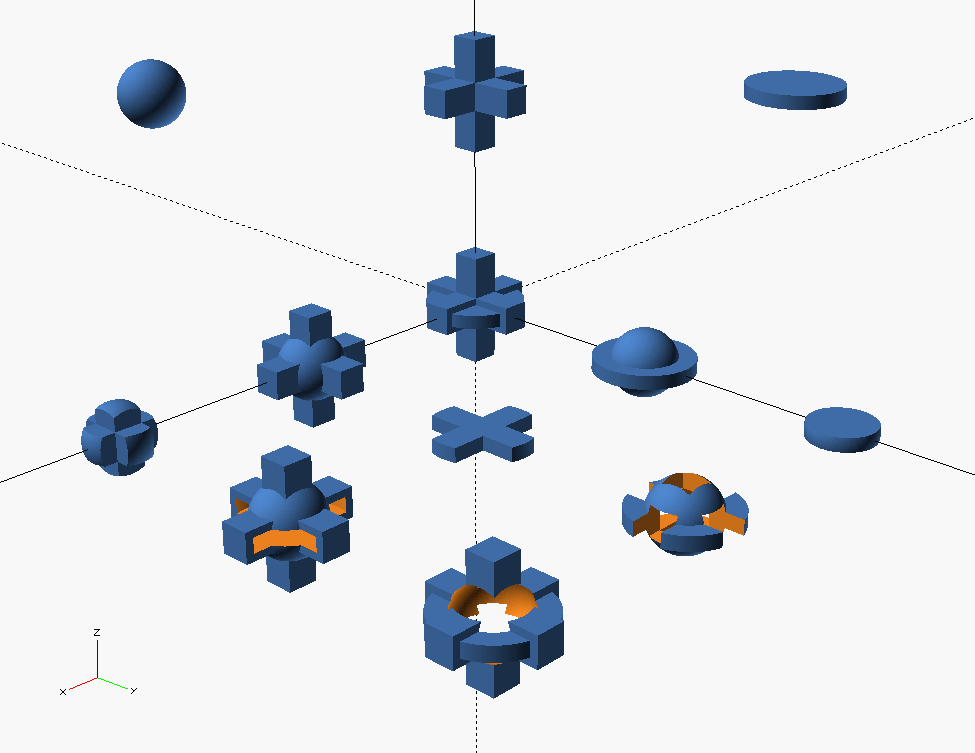
\includegraphics[scale=.375]{../figures/set_ops.png}

\newpage

\item What interval would the following infinite union be equal to?

\[ \bigcup_{n=2}^{\infty} [1, n] \]

\vfill

\item Let $D_n$ be the set of all positive integers that are divisors of $n$,

\[ D_N \; = \; \{ x \in \Integers^+ \suchthat \; x \divides n \}. \]

\noindent What is the following infinite intersection?

\[ \bigcap_{n=1}^{\infty} D_n \]

\vfill

\newpage

\item Here's a proof of the commutative property for $\cup$:

\begin{thm*}
For all sets $A$ and $B$, $A \cup B \; = \; B \cup A$.
\end{thm*}

\begin{proof}
We need to show that $x \in A \cup B \; \iff \; x \in B \cup A$. Suppose $A$ and $B$ are sets and $x$ is a particular but arbitrary element of
the universe of discourse.
\begin{align*}
 &      & x \in A \cup B \rule{48pt}{0pt} & \mbox{Given} & \\
 & \iff & x \in A \, \lor \, x \in B \rule{48pt}{0pt}  & \mbox{Definition of union} & \\
 & \iff & x \in B \, \lor \, x \in A \rule{48pt}{0pt}  & \mbox{Commutative property of disjunction} & \\
 & \iff & x \in B \cup A \rule{48pt}{0pt}  & \mbox{Definition of union} & 
\end{align*}
\end{proof}

Write a proof of the associative property for intersection.

\vfill

\vfill

\newpage

\item Here's a proof of the associative law for union. (It may be instructive to compare this to your answer on the last question.)

\begin{thm*}
For all sets $A$, $B$, and $C$, $(A \cup B) \cup C \; = \; A \cup (B \cup C)$.
\end{thm*}

\begin{proof}
We need to show that $x \in (A \cup B) \cup C) \; \iff \; x \in A \cup (B \cup C)$. Suppose $A$, $B$ and $C$ are sets and $x$ is a particular but arbitrary element of
the universe of discourse.
\begin{align*}
 &      & x \in (A \cup B) \cup C \rule{48pt}{0pt} & \mbox{Given} & \\
 & \iff & x \in (A \cup B) \lor x \in C \rule{48pt}{0pt}  & \mbox{Definition of union} & \\
 & \iff & (x \in A \lor x \in B) \lor x \in C \rule{48pt}{0pt}  & \mbox{Definition of union} & \\
 & \iff & x \in A \lor (x \in B \lor x \in C) \rule{48pt}{0pt}  & \mbox{Associative property of disjunction} & 
 & \iff & x \in A \lor (x \in B \cup C) \rule{48pt}{0pt}  & \mbox{Definition of union} & \\
  & \iff & x \in A \cup (B \cup C) \rule{48pt}{0pt}  & \mbox{Definition of union} & 
\end{align*}
\end{proof}

Now you try one! Prove the distributive law of union over intersection.

\vfill


\newpage
\item Do a quick review of your last two proofs with the following in mind:  On either side of a logical connector ($\land$ and $\lor$) we must find logical {\em statements} (like $x \in A$ or $x \in B$).  On either side of a set connector ($\cap$ and $\cup$) we must find {\em sets}!  

\vfill

\item Without referring back to the lecture video, do the activity of assembling the two column proof that
$A \triangle B \; = \; (A \cup B) \setminus (A \cap B)$ from the scrambled steps from page 184.

\vfill

\hspace{-1.1in}
\begin{tabular}{|c|l|}\hline
\rule[-18pt]{0pt}{48pt}$= (A \cap \overline{B}) \cup (B \cap \overline{A})$ & \rule{12pt}{0pt} identity law \\\hline
\rule[-18pt]{0pt}{48pt}$= (A \cup B) \cap \overline{(A \cap B)}$ & \rule{12pt}{0pt} def. of relative difference \rule{12pt}{0pt} \\\hline
\rule[-18pt]{0pt}{48pt}$(A \cup B) \setminus (A \cap B)$ & \rule{12pt}{0pt} Given  \\\hline
\rule[-18pt]{0pt}{48pt}\rule{12pt}{0pt}$= ((A \cap \overline{A}) \cup (A \cap \overline{B})) \cup ((B \cap \overline{A}) \cup (B \cap \overline{B}))$ \rule{12pt}{0pt} & \rule{12pt}{0pt} distributive law  \\\hline
\rule[-18pt]{0pt}{48pt}$= (A \setminus B) \cup (B \setminus A)$ & \rule{12pt}{0pt}  def. of relative difference \\\hline
\rule[-18pt]{0pt}{48pt}$= (A \cap \overline{(A \cap B)}) \cup (B \cap \overline{(A \cap B)})$ & \rule{12pt}{0pt} distributive law \\\hline
\rule[-18pt]{0pt}{48pt}$= A \triangle B $ & \rule{12pt}{0pt} def. of symmetric difference \rule{12pt}{0pt}\\\hline
\rule[-18pt]{0pt}{48pt}$= (A \cap (\overline{A} \cup \overline{B}) \cup (B \cap (\overline{A} \cup \overline{B}))$ & \rule{12pt}{0pt} DeMorgan's law \\\hline
\rule[-18pt]{0pt}{48pt}$= (\emptyset \cup (A \cap \overline{B})) \cup ((B \cap \overline{A}) \cup \emptyset)$ & \rule{12pt}{0pt} complementarity \\\hline
\end{tabular}


\end{enumerate}


\end{document}
